\section{Programovatelné logické obvody}
-CPLD, FPGA, struktury, rozdíly, použití, výhody,nevýhody
\subsection{CPLD - Complex Programmable Logic Devices}
CPLD se skládá ze sady programovatelných funkčních bloků. V každém bloku jsou makrobuňky. Makrobuňky jsou hlavními stavebními prvky CPLD. Vstupy a výstupy funkčních bloků jsou propojeny prostřednictvím globální propojovací matice (GIM). Tato propojovací matice je rekonfigurovatelná, takže není možné měnit kontakty mezi funkčními bloky. Tyto funkční bloky jsou podobné poli logických hradel.

Při návrhu CPLD je důležité věnovat pozornost technologii programování a funkčním blokům. Celkově jsou CPLD nevolatilní a snadno použitelné. Navíc jsou cenově výhodné.

PLD-programmable logic device. Obvody PLD realizují kombinaci logických funkcí
pomocí struktur SOP-sum of products čili součet součinů, resp. POS-product of sums čili
součin součtů. PLD obvody můžeme rozdělit do 3 skupin.

Klasické PLD obvody; každá vodorovná čára představuje součinové hradlo. Dělí se na
PROM, PLA a PAL obvody.

Komplexní PLD, CPLD; na rozdíl od klasických PLD obvodů umožňují realizovat i
složitější funkce. Jedná se vlastně o více PLD obvodů spojených dohromady.

V závislosti na tom, který prvek(který typ hradla) je
programovatelný dělíme obvody PLD do 3 struktur.
\textbf{Struktura PROM;} stupeň AND má zapojen napevno, stupeň OR je programovatelný.

\textbf{Struktura PAL}; stupeň AND je programovatelný, stupeň OR je zapojen napevno.
Struktura PAL je úspornější než PROM, protože v první části obvodu se vytvoří pouze ty
kombinace, které jsou skutečně potřebné pro realizaci funkce. Obvody PAL jsou užívány
častěji než PROM.

\textbf{Struktura PLA;} oba stupně AND a OR jsou programovatelné. Ze všech 3 metod je
nejúspornější. Kvůli velkému počtu programovatelných propojení nebyli tyto obvody
v době vývoje PLD obvodů úspěšné. Dnes se díky pokročilým technologiím začínají opět
objevovat.

    \begin{figure}[h]
   \begin{center}
     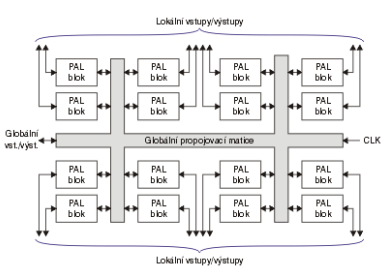
\includegraphics[scale=0.4]{images/CPLD.png}
   \end{center}
   \caption{CPLD}
  \end{figure}
  
      \begin{figure}[h]
   \begin{center}
     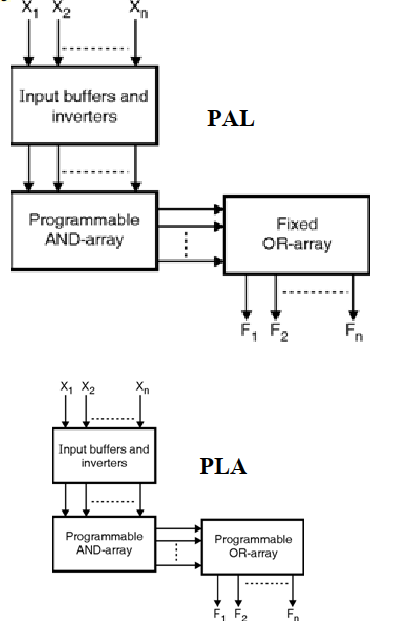
\includegraphics[scale=0.4]{images/PAL.png}
   \end{center}
   \caption{PAL a PLA}
  \end{figure}



\subsection{FPGA}
FPGA-field programmable gate array; z programovatelných obvodů mají nejvíce
logických hradel v jednom obvodě až 6 milionů hradel typově jako dvouvstupový NAND.
IOB input/output block představují vstupně výstupní obvody. LB jsou programovatelné
logické bloky

Uživatelé mohou navrhnout obvod pomocí jazyka pro popis hardwaru a nakonfigurovat jej tak, aby prováděl jednoduché hradlo, jako je hradlo AND, nebo složitý systém, jako je vícejádrový procesor. Všechny konfigurace ukládá do paměti RAM. Proto může výpadek napájení tyto konfigurace vymazat.

je pravděpodobné, že se budou stále více používat v chytrých telefonech a počítačích pro aplikace umělé inteligence a strojového učení. Rekonfigurovatelná povaha těchto čipů poskytuje vyhrazené zpracování pro složité algoritmy, aniž by spotřebovávala výpočetní zdroje, které jsou v těchto zařízeních vyhrazeny pro základní funkce.

Dokud nebudou FPGA optimalizovány pro masovou výrobu, zůstanou pravděpodobně ve většině zařízení vzácností. Pokud hledáte vysokou rychlost, nižší cenu a nižší spotřebu energie, může být lepší volbou aplikačně specifický integrovaný obvod (ASIC). Obětujete sice přizpůsobivost, ale vyhrajete díky nižším nákladům na velkosériové provozování zařízení.

Nevýhodou použití ASIC je nutná počáteční investice. Protože hardware není rekonfigurovatelný, budete se muset spojit se slévárnou, která váš ASIC vyrobí a zabalí. Po počátečních nákladech však mají ASIC nižší náklady na výrobu jedné jednotky, což z nich činí lepší volbu pro velkosériovou výrobu.

    \begin{figure}[h]
   \begin{center}
     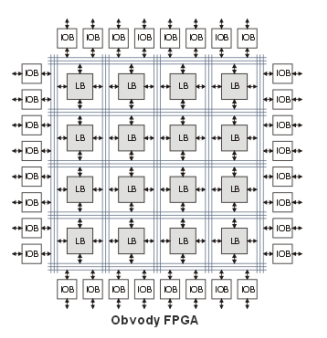
\includegraphics[scale=0.6]{images/FPGA.png}
   \end{center}
   \caption{FPGA}
  \end{figure}

\subsection{Rozdíly}  
Logické zdroje jsou také hlavním rozdílem mezi CPLD a FPGA. CPLD poskytuje minimum logických prostředků, zatímco FPGA poskytuje obrovské množství logických prostředků a paměťových prvků pro vytváření složitých systémů.\\
CPLD jsou cenově výhodné, ale FPGA jsou dražší než CPLD.\\
CPLD se skládají z větších bloků, zatímco FPGA se skládají z malých logických bloků.\\
Dalším rozdílem mezi CPLD a FPGA je jejich paměť. CPLD používá EEPROM (nevolatilní), zatímco FPGA používá RAM (volatilní).\\
Kromě toho je snazší předvídat zpoždění v CPLD než v FPGA.\\
 CPLD spotřebovává málo energie, zatímco FPGA spotřebovává více energie.\\
 CPLD je bezpečnější než FPGA, protože má zabudovanou nestálou paměť.\\
 CPLD je vhodný pro malé až středně velké aplikace, zatímco FPGA je vhodný pro složité aplikace.\\
  
  
  
  
  
  
  
  
  
  
  
  
  